\begin{proof}
Soit $C$ une courbe. 
Soit $\epsilon>0$.
\[\A=\inf \enstq{B(i, \frac{\epsilon}{2})}{C\subset \bigcup_{icIcR2} B(i, \frac{\epsilon}{2})}\]
On note \[N_\epsilon =card(A)\]
Soit \[M_a (C)=lim_{\epsilon\rightarrow0}(N_\epsilon\epsilon^{a}), a\geq0 \textm{la mesure de Hausdorff} \]
On note: \[D_{H}(\mathcal{C})=inf_{IR+} \enstq{a}{Ma(\mathcal{C})=0}\]
Soit $\mathcal{Q}$ un quadrillage dont les cases, (notées $Q_{ij}, i,j e Z$) ont pour côté $\epsilon$.
Soit \[\mathcal{A'}= \enstq{Q_{ij}}{\mathcal{C}\subset \bigcup_{i,j e Z^{2}}Q_{ij}}\]
On note \[N'_{\epsilon}=card(\mathcal{A'})\]
Soit \[\mathcal{M}_{a}'(\mathcal{C})=lim_{\epsilon\rightarrow0}(N'_\epsilon\epsilon^{a})\]
On note: \[D_{H}'(\mathcal{C})=inf_{IR+} \enstq{a}{Ma'(\mathcal{C})=0}\]
On veut montrer que pour un $\mathcal{C}$ donné, \[D_{H}(\mathcal{C})=D_{H}'(\mathcal{C})
\textm{c'est à dire :}  \forall a \in IR+, \mathcal{M}_{a}(\mathcal{C})=0\Leftrightarrow \mathcal{M}_{a}'(\mathcal{C})\]
$\Longrightarrow$/ Prouvons maintenant que \[\mathcal{M}_{a}(\mathcal{C})=0 \Rightarrow \mathcal{M}_{a}'(\mathcal{C})
\textm{c'est à dire} \lim \limits_{\epsilon \rightarrow 0}(N_\epsilon\epsilon^{a})=0 \Rightarrow lim_{\epsilon\rightarrow0}(N'_\epsilon\epsilon^{a})=0\]
Or \[\exists>0 | N'_{\epsilon} \leq cN_{\epsilon} \Rightarrow lim_{\epsilon\rightarrow0}(N_\epsilon\epsilon^{a})=0 \Rightarrow lim_{\epsilon\rightarrow0}(N'_\epsilon\epsilon^{a})=0\]
Or, \[\forall\epsilon > 0, N'_{\epsilon} \leq 4N_{\epsilon}\]
\begin{figure}[h]
\centering
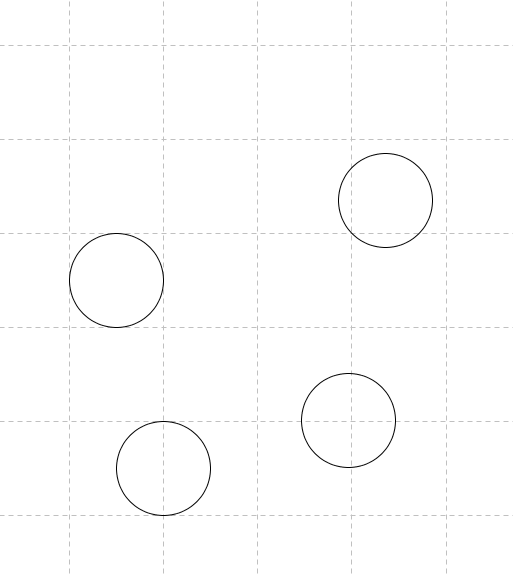
\includegraphics[width=10cm]{cases.png}
\caption{$\forall\epsilon > 0, N'_{\epsilon} \leq 4N_{\epsilon}$}
\label{fig:cases}
\end{figure}
Donc \[lim_{\epsilon\rightarrow0}(N'_\epsilon\epsilon^{a}) \leq lim_{\epsilon\rightarrow0}(4N_\epsilon\epsilon^{a})\]
c'est à dire\[lim_{\epsilon\rightarrow0}(N'_\epsilon\epsilon^{a}) \leq 4lim_{\epsilon\rightarrow0}(N_\epsilon\epsilon^{a})\]
c'est à dire \[lim_{\epsilon\rightarrow0}(N'_\epsilon\epsilon^{a}) \leq 0 \textm{(par hypothèse)}\] 
Or 
\begin{equation*}\label{y}
\begin{split}
N_\epsilon \geq 0 \textm{et} \epsilon \geq 0 & \Rightarrow 0 \leq \lim\limits_{\epsilon \Rightarrow 0} (N'_\epsilon\epsilon^{a}) \leq 0 \\
& \Rightarrow \lim\limits_{\epsilon \Rightarrow 0} (N'_\epsilon\epsilon^{a}) = 0 \textm{selon le théorème de l'encadrement}
\end{split}
\end{equation*}
Ainsi: \[\mathcal{M}_{a}(\mathcal{C})=0 \Rightarrow \mathcal{M}_{a}'(\mathcal{C})=0 \]
$\Longleftarrow$/ Montrons que \[\mathcal{M}_{a}(\mathcal{C})=0 \Leftarrow \mathcal{M}_{a}'(\mathcal{C})\]
\[\lim\limits{\epsilon\rightarrow0}(N_{\epsilon}\epsilon^{a})=0 \Leftarrow lim_{\epsilon\rightarrow0}(N'_{\epsilon}\epsilon^{a})=0\]
D'après la proposition \[\exists c' | N_{c\epsilon} \leq N\epsilon' \Rightarrow (lim_{\epsilon\rightarrow0}(N'_\epsilon\epsilon^{a})=0 \Rightarrow lim_{\epsilon\rightarrow0}(N_\epsilon\epsilon^{a})=0\]
Or \[N_{\sqrt[]{2}\epsilon} \leq N'_{\epsilon}\]
Ainsi \[\lim\limits{\epsilon\rightarrow0}(N_{\sqrt[]{2}\epsilon}(\sqrt[]{2}\epsilon)^{a}) \leq \sqrt[]{2}^{a}lim_{\epsilon\rightarrow0}N'_{\epsilon}\epsilon^{a}\]
Or \[N_{\sqrt[]{2}\epsilon} \geq 0 et (\sqrt[]{2}\epsilon)^{a} \geq0\]
On note \[\epsilon'=\sqrt[]{2}\epsilon\]
On voit que \[\epsilon'\rightarrow0 \Leftrightarrow \epsilon\Rightarrow0\]
Donc \[\lim\limits{\epsilon\rightarrow0}(N_{\epsilon}\epsilon^{a})=lim_{\epsilon\rightarrow0}(N'_{\epsilon}\epsilon'^{a})=0\]
Ainsi \[\mathcal{M}_{a}(\mathcal{C})=0 \Leftrightarrow \mathcal{M}_{a}'(\mathcal{C}) \]
Donc \[\inf_{IR+}{\enstq{a}{M'_{a}(\mathcal{C})=0}}= \inf_{IR+}{\enstq{a}{M_{a}(\mathcal{C})=0}}\]
Donc \[\mathcal{D}_{H}(\mathcal{C})=\mathcal{D}'_{H}(\mathcal{C})\]
\end{proof}